\documentclass[11pt]{article}
\usepackage[margin=0.9in]{geometry}
\usepackage{graphicx}
\usepackage{xcolor}
\usepackage{parskip}
\usepackage{enumitem}
\usepackage[T1]{fontenc}
\usepackage{helvet}
\renewcommand{\familydefault}{\sfdefault}
\usepackage[hidelinks]{hyperref}

\graphicspath{{diagrams/overview/}}
\setlength{\parskip}{6pt}
\definecolor{ink}{HTML}{1F2A37}
\definecolor{soft}{HTML}{5A6B82}
\definecolor{boxbg}{HTML}{EEF3FA}
\definecolor{boxln}{HTML}{3B5B92}
\color{ink}

% simple "in plain terms" callout
\newcommand{\plainbox}[1]{%
  \par\vspace{2pt}\noindent
  \fcolorbox{boxln}{boxbg}{\parbox{\dimexpr\linewidth-2\fboxsep-2\fboxrule}{\small #1}}%
  \par\vspace{2pt}}

\newcommand{\heading}[1]{\vspace{4pt}\par{\large\bfseries #1}\par\vspace{-2pt}}

\begin{document}
\thispagestyle{empty}

\begin{center}
{\LARGE\bfseries Leg-Entanglement Detection \& Recovery}\\[4pt]
{\large Project Overview}\\[6pt]
{\color{soft}\itshape A plain-language summary for a non-technical reader}
\end{center}

\vspace{2pt}
\plainbox{\textbf{In one sentence:} we built software that lets a four-legged robot notice
--- in real time, from its own body sensors --- when one of its legs gets caught on a wire,
net, or a person's hand, tell \textbf{which} leg and \textbf{how badly}, and then attempt to
free it safely.}

\heading{1.\quad The problem}
Four-legged robots increasingly work in messy, real-world spaces: rooms with cables, outdoor
sites with netting or vegetation, or alongside people who might grab a leg. When a leg gets
\textbf{caught}, the robot keeps trying to walk and fights the obstacle --- and within a
second or two it can stumble or fall. A fall means downtime, damage, and a safety risk.

Spotting this early is surprisingly hard:
\begin{itemize}[leftmargin=1.4em,itemsep=1pt,topsep=2pt]
  \item \textbf{Cameras don't help much.} Thin wires and clear line are nearly invisible, and
  the robot's own body blocks the view of its legs.
  \item \textbf{A simple rule doesn't work.} The warning sign is subtle --- a small, brief
  change in how hard a leg is straining --- and it looks a lot like normal walking, standing,
  or the stiff pose the robot holds right after standing up. One fixed threshold either misses
  real snags or cries wolf constantly.
\end{itemize}

So instead of a camera or a fixed rule, we use the robot's \textbf{own sense of touch} --- the
hundreds of force and motion readings its legs already produce every second --- and a small
\textbf{trained model} that has learned what a real snag looks like.

\heading{2.\quad Our solution}
The system runs as a continuous loop on the robot, in four simple steps:

\begin{center}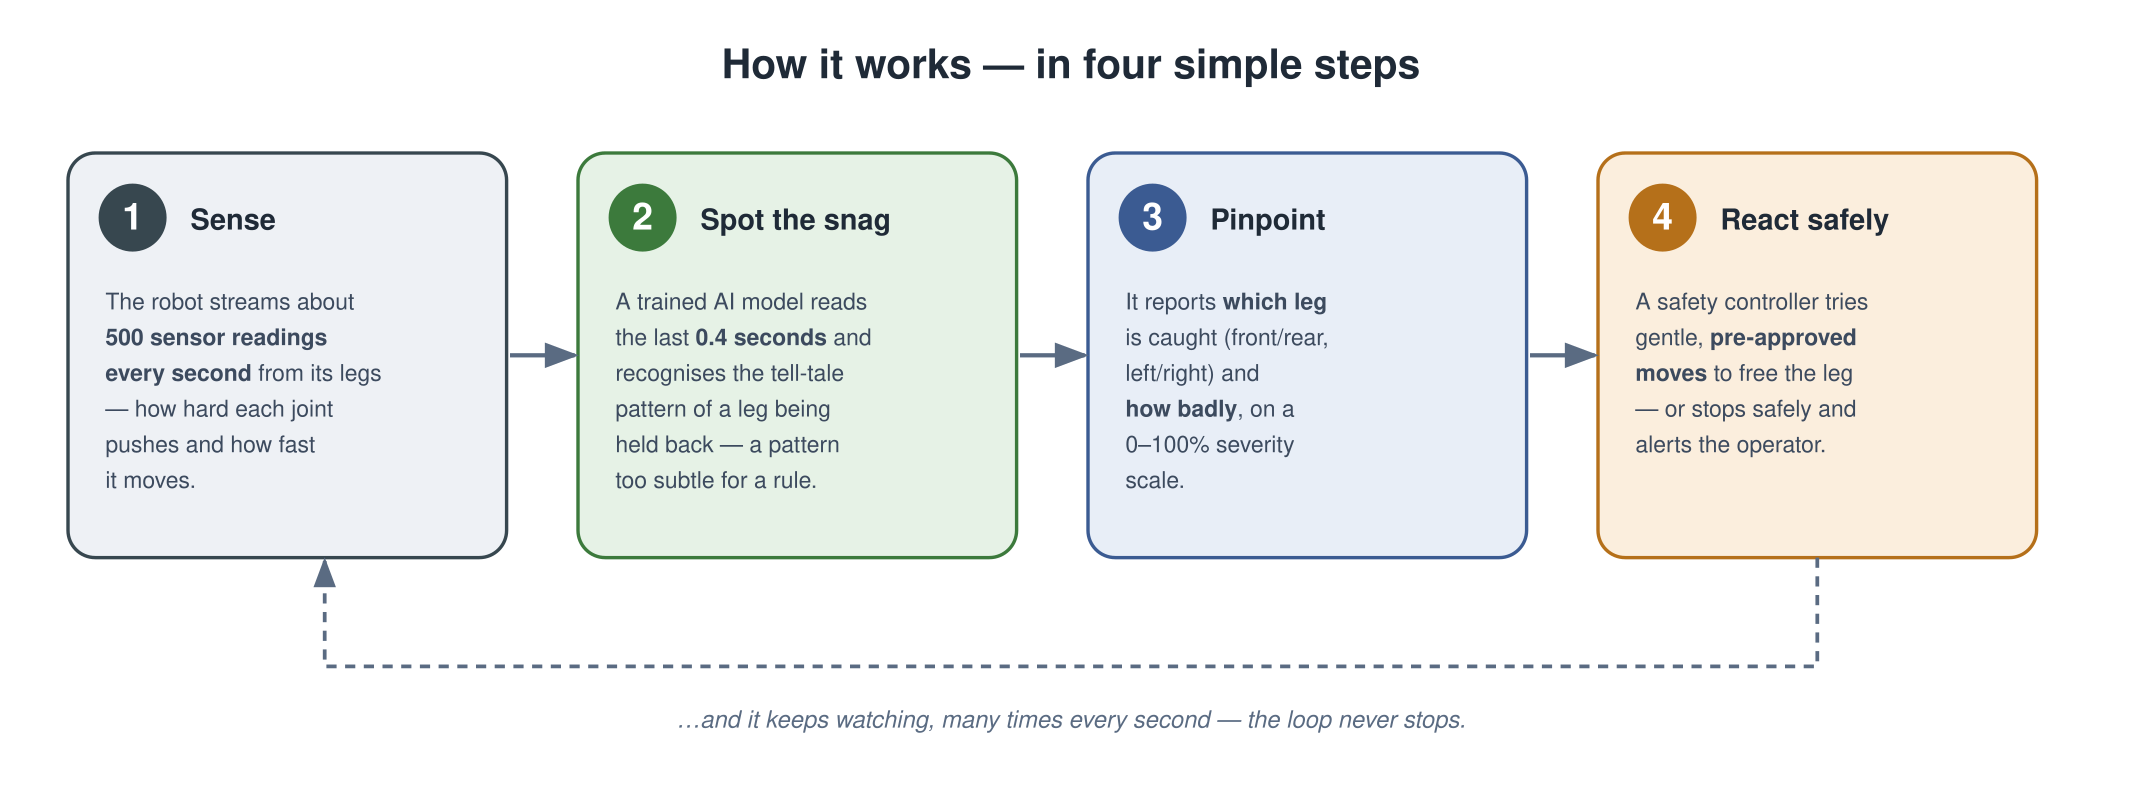
\includegraphics[width=\linewidth]{flow_simple.png}\end{center}

\plainbox{\textbf{What is the ``AI model''?} Think of it as a pattern-recogniser that we
\emph{taught} by showing it many real examples --- recordings where a leg was caught, and
recordings of normal walking, standing, and stopping. It learned the difference on its own,
so it catches subtle cases a hand-written rule would miss. It only ever looks at the recent
past, so it can run live on the robot.}

The step that makes the system genuinely useful is \textbf{Step 3}: at every instant it
reports \emph{which} leg is caught and \emph{how badly}.

\begin{center}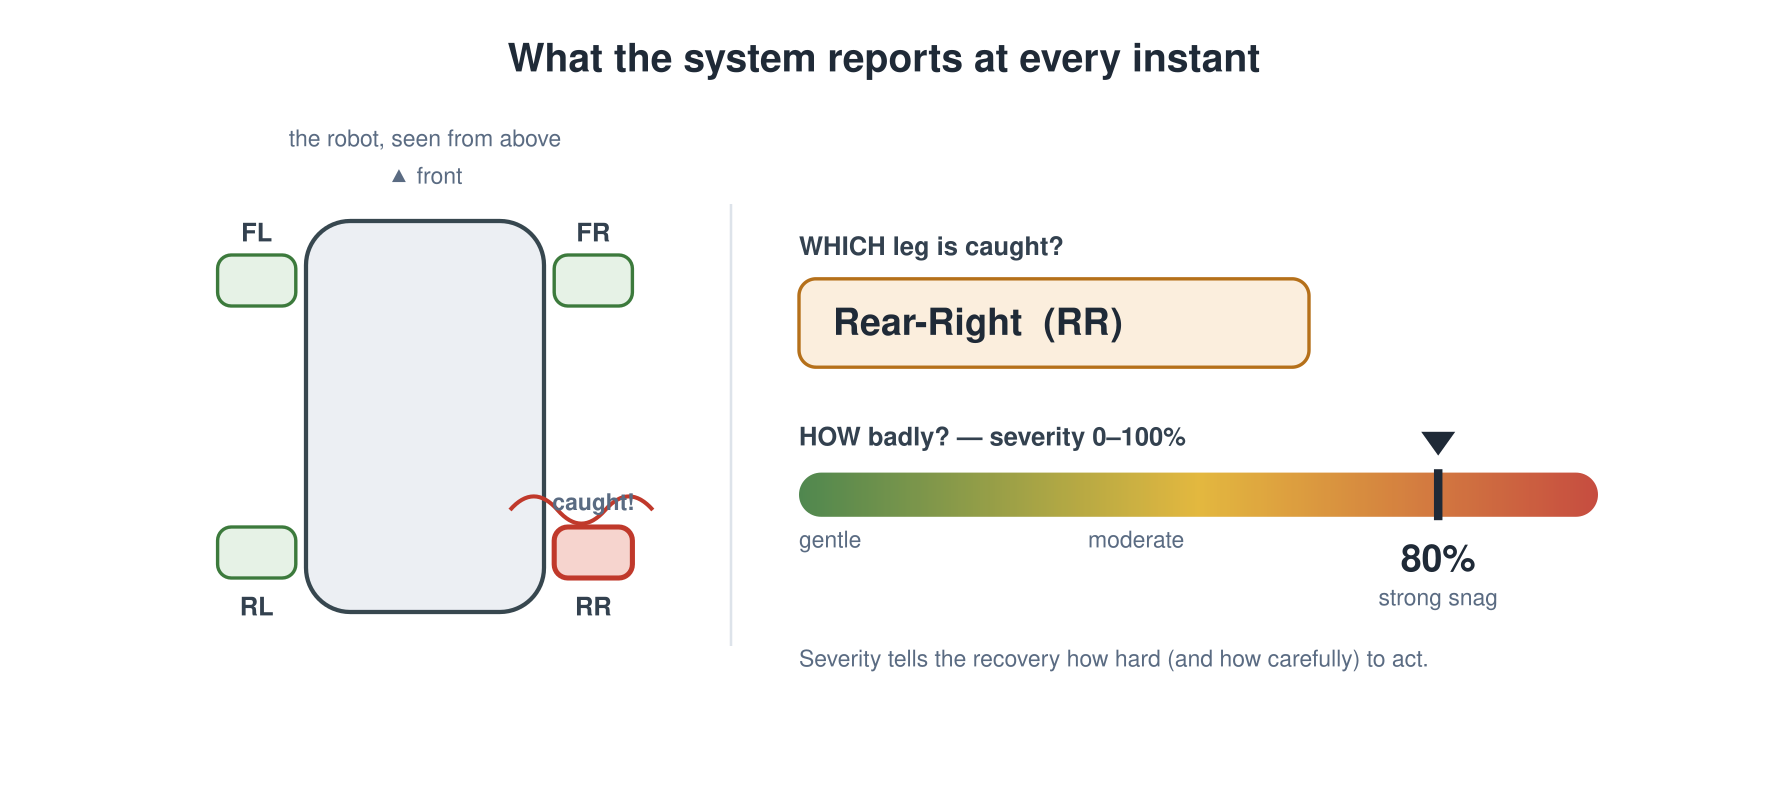
\includegraphics[width=\linewidth]{what_it_tells.png}\end{center}

In \textbf{Step 4}, a separate \textbf{safety controller} uses that information to try gentle,
pre-approved moves to free the leg --- or stops the robot safely and alerts the operator. This
recovery ships \textbf{switched off by default} and only logs what it \emph{would} do, so it
can be checked thoroughly before it is ever allowed to move a real robot. We deliberately kept
the model \textbf{small and fast} so it runs on the robot's own modest computer in about a
thousandth of a second, with no extra hardware and no network dependency.

\heading{3.\quad Results --- and what's new}
\begin{center}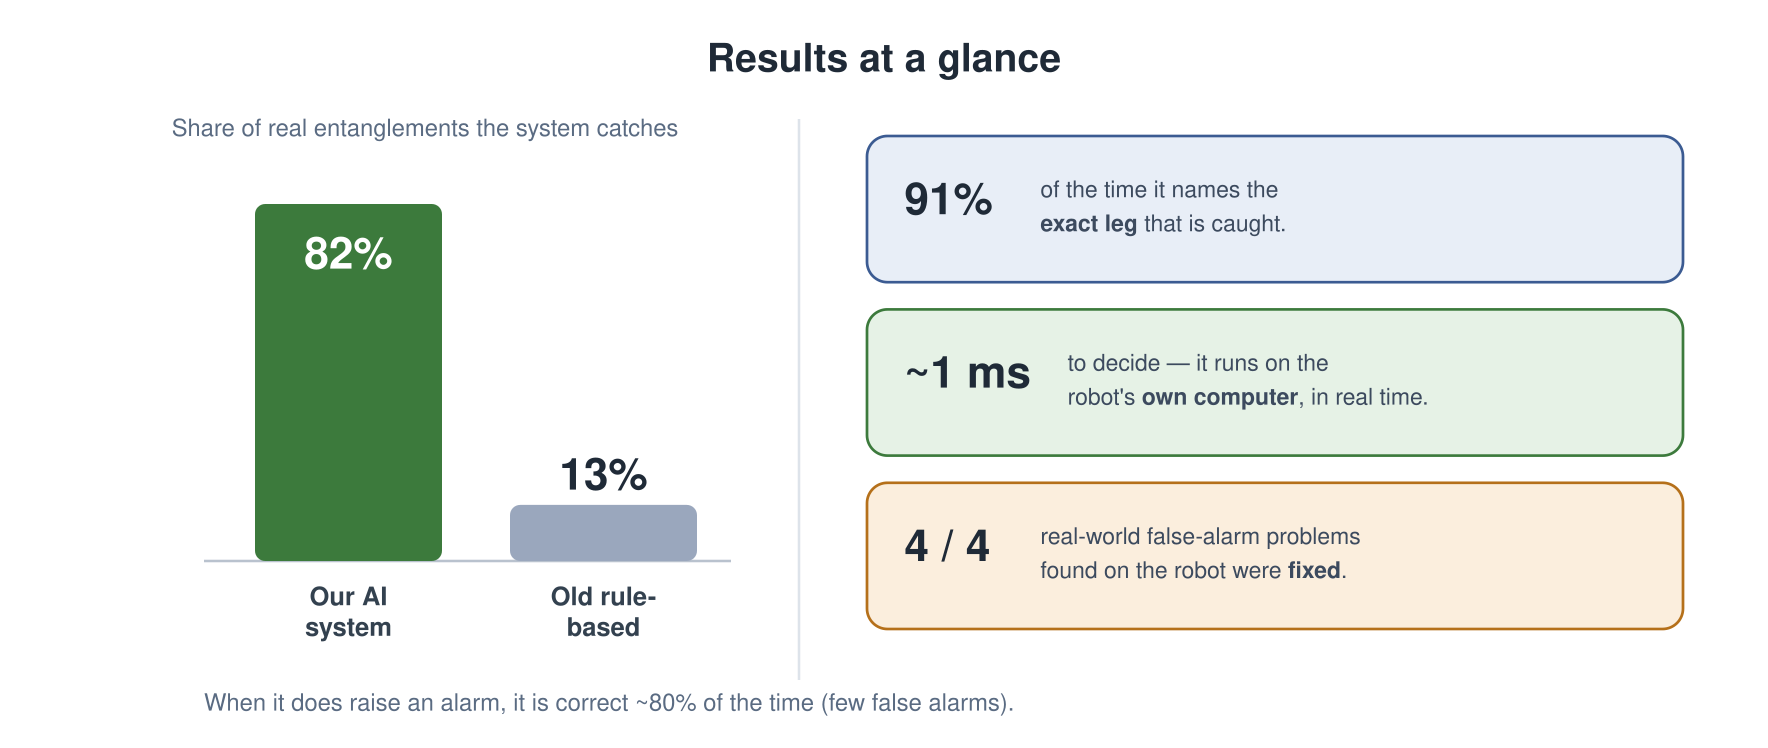
\includegraphics[width=\linewidth]{results_simple.png}\end{center}

Measured carefully on held-out data the model had never seen during training:
\begin{itemize}[leftmargin=1.4em,itemsep=1pt,topsep=2pt]
  \item It \textbf{catches about 82\%} of real entanglements --- versus only \textbf{13\%}
  for the older, rule-based approach on the same data.
  \item When it \emph{does} raise an alarm, it is \textbf{correct about 80\%} of the time.
  \item It names the \textbf{exact leg} correctly about \textbf{91\%} of the time.
  \item It decides in about \textbf{1 millisecond} on the robot's own CPU --- real-time.
  \item After the first on-robot trial we found \textbf{four} false-alarm situations
  (e.g.\ right after standing up, or walking backwards); a little more data and re-training
  \textbf{eliminated all four}.
\end{itemize}

\textbf{What makes this novel.} Most prior work answers only \emph{``is a leg caught?''}. Our
system adds the two things a recovery controller actually needs:

\textbf{(a) The exact leg}, not just ``a leg''. The model points to one of the four specific
legs, which tells the recovery \emph{where} to act. We score this strictly --- it must name
exactly the right leg --- and it succeeds $\sim$91\% of the time.

\textbf{(b) A severity score (0--100\%) --- ``how badly''.} There are no ready-made severity
measurements to learn from, so we compute severity from \textbf{physics}, blending two
intuitive signals for the flagged leg:
\begin{enumerate}[leftmargin=1.6em,itemsep=1pt,topsep=2pt]
  \item \textbf{Strain-without-motion} --- how hard the leg pushes while barely moving. A leg
  that pushes hard but goes nowhere is being held by \emph{something}.
  \item \textbf{How unusual the motion looks} --- how far the leg's behaviour has drifted from
  normal walking.
\end{enumerate}
These combine into one score that sits near \textbf{0\% in normal walking/standing} and
\textbf{rises smoothly as a snag worsens}. The recovery uses it to act gently for a light
pinch and more cautiously for a strong snag.

\textbf{The system in action.} Below is a real recording of a front-right leg caught on a
wire. At the snag, all three outputs light up together --- the alarm, the correct leg, and the
severity --- and fall back to zero the moment the leg is released; the other legs stay quiet.

\begin{center}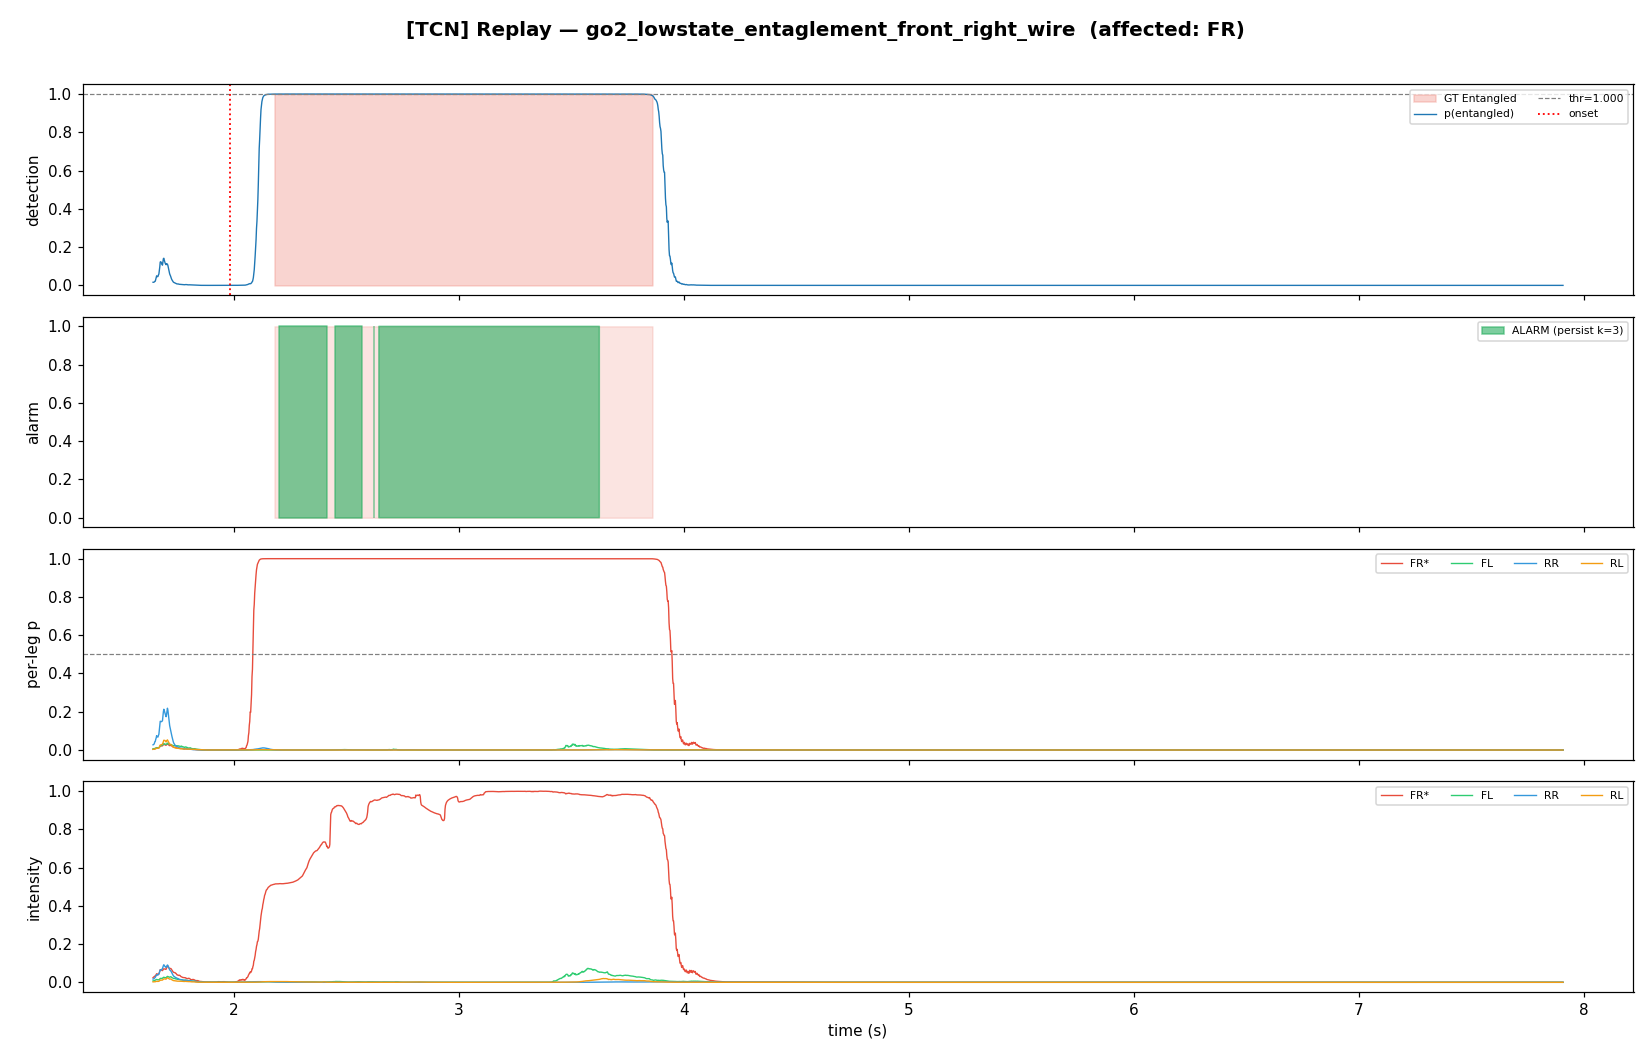
\includegraphics[width=0.96\linewidth]{system_in_action.png}\end{center}
{\small\color{soft} Top to bottom: alarm confidence; the alarm; which leg (front-right, red);
and severity --- all rising at the snag and clearing at release.}

\heading{4.\quad Safety by design}
\begin{itemize}[leftmargin=1.4em,itemsep=1pt,topsep=2pt]
  \item \textbf{Off by default.} Recovery motion is disabled unless an operator turns it on;
  otherwise it only \emph{logs} what it would do.
  \item \textbf{Only pre-approved moves} from the manufacturer's own documented commands, so
  the robot stays within its built-in balance limits.
  \item \textbf{Always a safe exit:} an emergency-stop makes the robot go limp instantly, and
  any fault or timeout falls back to that safe state automatically.
  \item \textbf{Detection is watch-only:} the detector never commands motion; it only reports.
\end{itemize}

\heading{5.\quad Where we are, and what's next}
\textbf{Proven so far (measured):} the detection accuracy, the exact-leg and severity outputs,
the real-time speed on the robot's CPU, and the elimination of the four field false-alarm
cases. The recovery decision-logic is fully tested in simulation.

\textbf{Still to validate on the real robot (honest caveat):} whether the recovery
\emph{moves} actually free a caught leg in practice --- the directions and strengths of those
moves are sensible engineering choices but have \textbf{not yet been proven on hardware}. That
is why recovery ships switched off. The next step is a staged robot trial: detector only
$\rightarrow$ recovery in log-only mode $\rightarrow$ carefully supervised live recovery.

\textbf{Biggest opportunity:} collect more examples of the under-represented cases (especially
front-right snags) --- the clearest way to push accuracy higher.

\vfill
{\footnotesize\color{soft} Prepared as a non-technical overview. A full technical write-up
(methods, metrics, and a formal paper) is available in the project repository for the
engineering team.}

\end{document}
